% Chapter 4

\chapter{Results} % Chapter title

\label{ch:results} % For referencing the chapter elsewhere, use \autoref{ch:introduction} 

%----------------------------------------------------------------------------------------
\section{List of Sources}
Twenty two sources were analysed; a full list is shown below. Results have been grouped according to suggested class of HMXB, and approximately in order of confidence.
\begin{itemize}
\item 1A0535+262
\item AXJ1910.7+0917
\item Cen X-3
\item EXO2030+375
\item IGRJ08408-4503
\item IGRJ11215-5952
\item IGRJ16418-4532
\item IGRJ16465-4507
\item IGRJ16479-4514
\item IGRJ17391-3021
\item IGRJ17407-2808
\item IGRJ17544-2619
\item IGRJ18027-2016
\item IGRJ18219-1347
\item IGRJ18410-0535
\item IGRJ18450-0435
\item IGRJ18483-0311
\item MAXIJ1409-619
\item OAO1657-415
\item SAXJ1818.6-1703
\item Vela X-1
\item XPer
\end{itemize}
\clearpage{}

\section{Supergiant X-ray Binaries}
\subsection{Cen X-3}

\begin{figure}[h!]
\centering
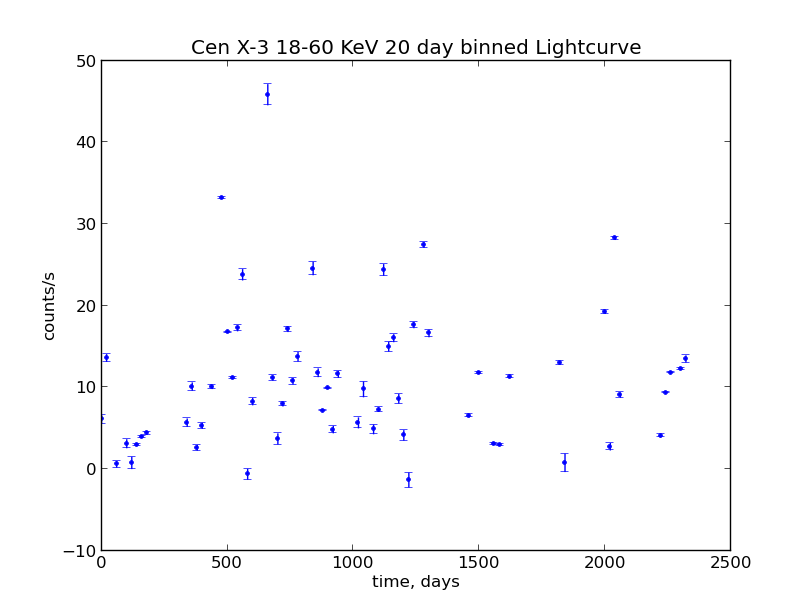
\includegraphics[width=130mm]{gfx/Fig7.png}
\caption{20 day binned lightcurve for Cen X-3.}
\label{Figure 7}
\end{figure}

Cen X-3 is a very bright and well studied source, and as it\textquoteright{}s designation would suggest, was one of the first X-ray sources to be discovered. It is a SGXB, and so is powered primarily by stellar wind loss. It has a well documented 2.087 day cycle.

\begin{figure}[h!]
\centering
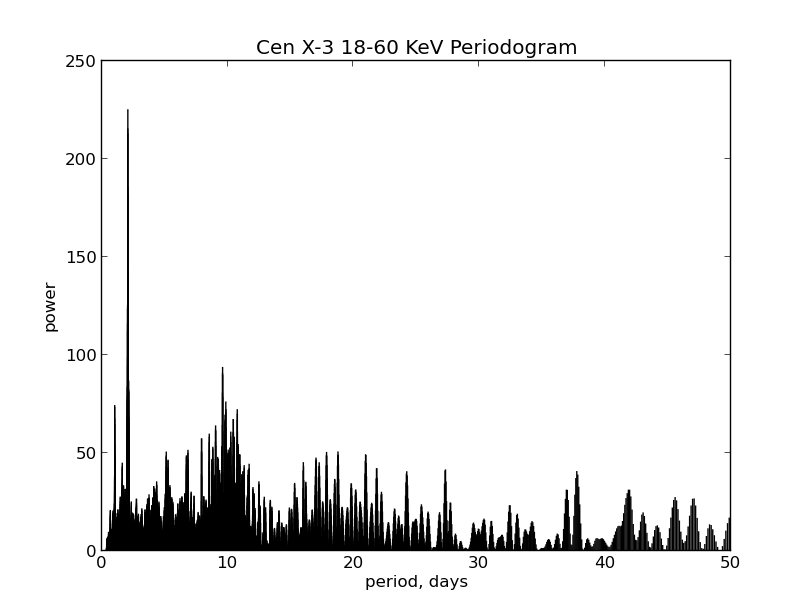
\includegraphics[width=130mm]{gfx/Fig8.png}
\caption{Periodogram for Cen X-3. The expected peak at 2.087 days is very clear.}
\label{Figure 8}
\end{figure}

\ref{Figure 7} shows a binned lightcurve. Although this does not reveal anything useful, it is an example of a particularly good source. Cen X-3 is very luminous, and the error bars and count rates reflect this. \ref{Figure 8} shows a periodogram from Cen X-3. The expected peak at 2.087 days is very clear. Once folded on this period, \ref{Figure 9} shows the eclipse profile. From these results, it is easy to see that Cen X-3 shows the behaviour expected of a SGXB. It is luminous and active except when eclipsing, and provides a good example to measure other less well known and more uncertain sources against. 

\begin{figure}[h!]
\centering
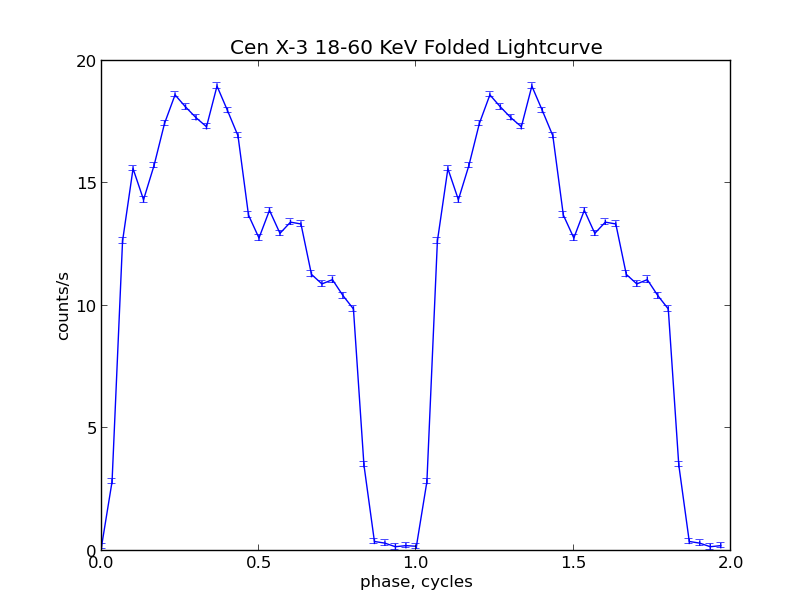
\includegraphics[width=130mm]{gfx/Fig9.png}
\caption{Folded lightcurve for Cen X-3.}
\label{Figure 9}
\end{figure} 

\clearpage
\subsection{Vela X-1}

\begin{figure}[h!]
\centering
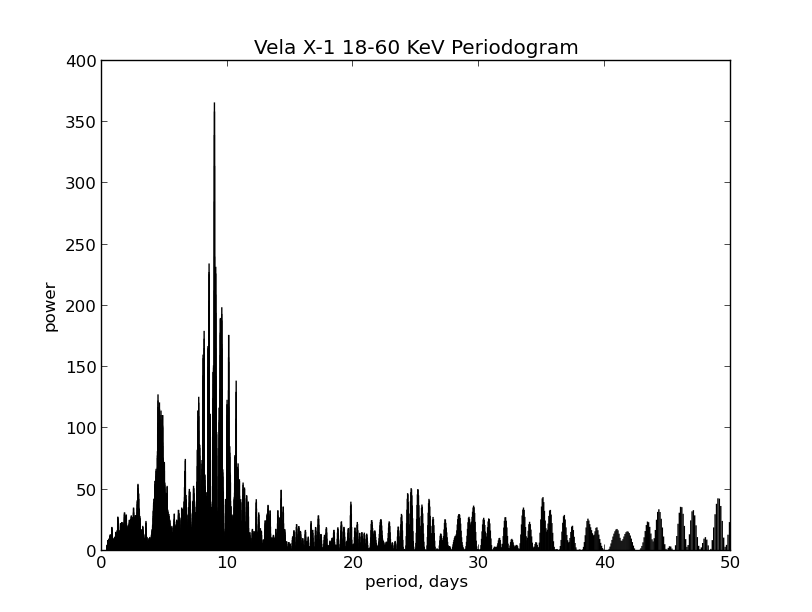
\includegraphics[width=130mm]{gfx/Fig10.png}
\caption{Periodogram for Vela X-1.}
\label{Figure 10}
\end{figure} 

Vela X-1 is another bright SGXB that was discovered early in the study of XRBs, and like Cen X-3 and Cyg X-1 could be considered a textbook example of it\textquoteright{}s class. The orbital period of the system is already known to be 8.964 days.

\ref{Figure 10} shows the periodogram, with a large peak at the expected 8.964 days. \ref{Figure 11} shows the folded light curve on that period, and the eclipse profile is shown convincingly. 

\begin{figure}[h!]
\centering
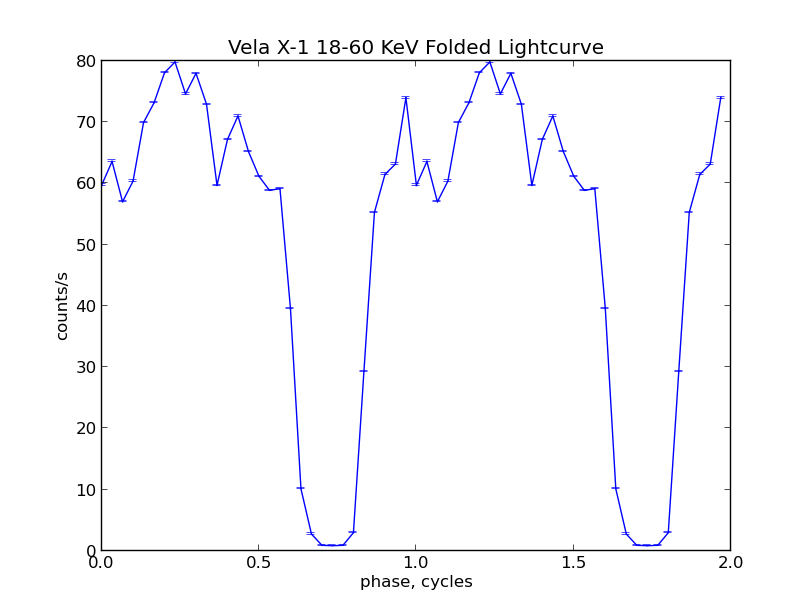
\includegraphics[width=130mm]{gfx/Fig11.png}
\caption{Folded lightcurve for Vela X-1. Period: 8.964 days.}
\label{Figure 11}
\end{figure} 

\subsection{OAO1657-415}
OAO1657-415 is very similar to both Vela X-1 and Cen X-3, and is another SGXB. It has a slightly longer known period of 10.4 days and it has been suggested that this source might not be entirely wind-fed, and that a proportion of the accretion may be through a disk. These results corroborate with the 10.4 day period, as shown in the periodogram \ref{Figure 12}, which peaks at 10.45 days. \ref{Figure 13} shows the folded lightcurve, and the eclipse, clearly showing that these results agree with the body of literature. 

\begin{figure}[h!]
\centering
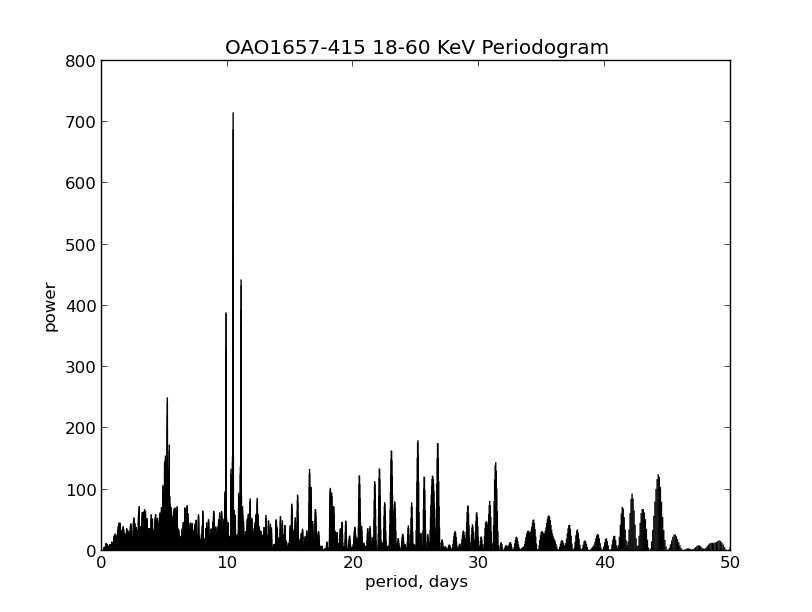
\includegraphics[width=130mm]{gfx/Fig12.png}
\caption{Periodogram for OAO1657-415. Peak at 10.45 days.}
\label{Figure 12}
\end{figure} 

\begin{figure}[h!]
\centering
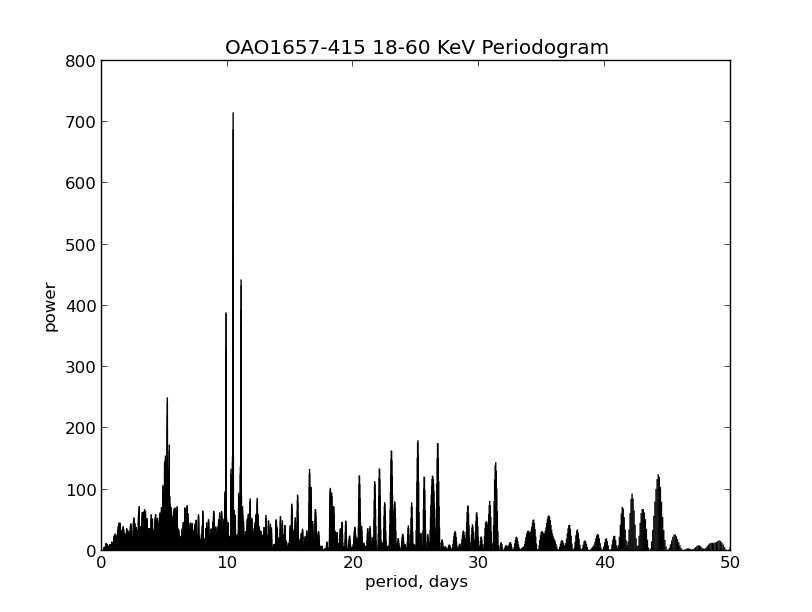
\includegraphics[width=130mm]{gfx/Fig12.png}
\caption{Folded lightcurve for OAO1657-415. Period: 10.45 days.}
\label{Figure 13}
\end{figure} 

\subsection{IGRJ18027-2016}
IGRJ18027-2016 is another probable Supergiant X-ray Binary, and was the test source used in this project. The results for this source were shown in the previous section. \ref{Figure 3} shows the periodogram, and \ref{Figure 5} shows the folded light curve and eclipse, with a period of 4.570 days. 

\clearpage

